\subsection{Plane earth signal budget} \label{sec:pepl}
Building on the free space signal budget, the plane earth signal budged now takes into account the Earth's surface as an infinitely extended smooth plane, with the antennas being mounted at heights $h_\mathrm{T}$ and $h_\mathrm{R}$ in $\left(\mathrm{m}\right)$ above this plane. As a result of this arrangement, the transmitted electromagnetic waves are now reflected in such a way that they can increase the available power $P_\mathrm{R}$ at the receiver. Figure \ref{fig:tikz_plane_earth_signal_budget} is used for illustration. An electromagnetic wave reflected from the ground covers the path $d_2$ in $\left(\mathrm{m}\right)$, whereas a wave that is transmitted directly from the transmission to the receiving antenna covers the path $d_1$ in $\left(\mathrm{m}\right)$. $\psi$ in $\left(^\circ\right)$ is the \emph{angle of incidence} of the electromagnetic waves at the point of reflection and $\underline{\rho}$ is the \emph{complex reflection coefficient for vertical polarization} in $\left(\mathrm{1}\right)$.
\begin{figure}[h!]
	\centering
	

\tikzset{every picture/.style={line width=0.75pt}} %set default line width to 0.75pt        

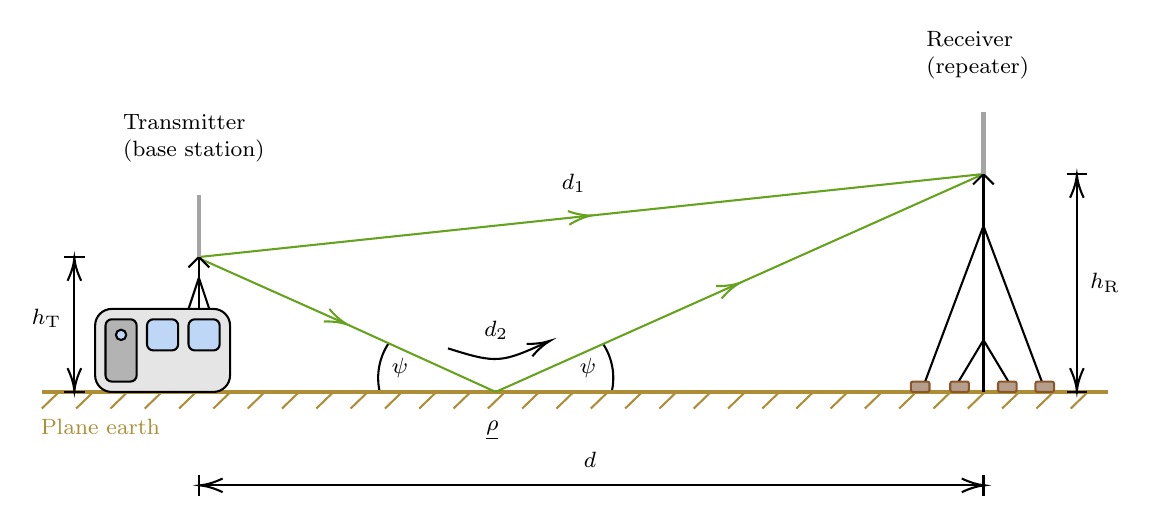
\begin{tikzpicture}[x=0.75pt,y=0.75pt,yscale=-1,xscale=1]
%uncomment if require: \path (0,876); %set diagram left start at 0, and has height of 876

%Shape: Arc [id:dp15338331881086464] 
\draw  [draw opacity=0] (340.87,690.02) .. controls (341.8,685.99) and (341.92,681.69) .. (341.05,677.36) .. controls (340.27,673.48) and (338.78,669.92) .. (336.73,666.79) -- (311.63,683.25) -- cycle ; \draw   (340.87,690.02) .. controls (341.8,685.99) and (341.92,681.69) .. (341.05,677.36) .. controls (340.27,673.48) and (338.78,669.92) .. (336.73,666.79) ;
%Shape: Arc [id:dp6996067112202611] 
\draw  [draw opacity=0] (229.13,689.98) .. controls (228.2,685.94) and (228.08,681.64) .. (228.95,677.32) .. controls (229.74,673.35) and (231.29,669.72) .. (233.4,666.55) -- (258.37,683.2) -- cycle ; \draw   (229.13,689.98) .. controls (228.2,685.94) and (228.08,681.64) .. (228.95,677.32) .. controls (229.74,673.35) and (231.29,669.72) .. (233.4,666.55) ;
%Straight Lines [id:da4849283455814688] 
\draw    (142,730) -- (142,740) ;
%Straight Lines [id:da7410756286600795] 
\draw    (520,730) -- (520,740) ;
%Straight Lines [id:da9884557143123041] 
\draw    (144.5,735) -- (518.5,735) ;
\draw [shift={(520.5,735)}, rotate = 180] [color={rgb, 255:red, 0; green, 0; blue, 0 }  ][line width=0.75]    (10.93,-3.29) .. controls (6.95,-1.4) and (3.31,-0.3) .. (0,0) .. controls (3.31,0.3) and (6.95,1.4) .. (10.93,3.29)   ;
\draw [shift={(142.5,735)}, rotate = 0] [color={rgb, 255:red, 0; green, 0; blue, 0 }  ][line width=0.75]    (10.93,-3.29) .. controls (6.95,-1.4) and (3.31,-0.3) .. (0,0) .. controls (3.31,0.3) and (6.95,1.4) .. (10.93,3.29)   ;
%Straight Lines [id:da6201954809627948] 
\draw [color={rgb, 255:red, 173; green, 142; blue, 55 }  ,draw opacity=1 ][fill={rgb, 255:red, 139; green, 87; blue, 42 }  ,fill opacity=1 ][line width=1.5]    (66.3,690) -- (430,690) ;
%Straight Lines [id:da06147530745502938] 
\draw [color={rgb, 255:red, 173; green, 142; blue, 55 }  ,draw opacity=1 ]   (74.59,690) -- (66.32,697.99) ;
%Straight Lines [id:da23007865791418336] 
\draw [color={rgb, 255:red, 173; green, 142; blue, 55 }  ,draw opacity=1 ]   (91.12,690) -- (82.85,697.99) ;
%Straight Lines [id:da767472737068108] 
\draw [color={rgb, 255:red, 173; green, 142; blue, 55 }  ,draw opacity=1 ]   (107.65,690) -- (99.38,697.99) ;
%Straight Lines [id:da13777850468332842] 
\draw [color={rgb, 255:red, 173; green, 142; blue, 55 }  ,draw opacity=1 ]   (124.18,690) -- (115.91,697.99) ;
%Straight Lines [id:da6751673575123742] 
\draw [color={rgb, 255:red, 173; green, 142; blue, 55 }  ,draw opacity=1 ]   (140.71,690) -- (132.44,697.99) ;
%Straight Lines [id:da9392755627171439] 
\draw [color={rgb, 255:red, 173; green, 142; blue, 55 }  ,draw opacity=1 ]   (157.24,690) -- (148.98,697.99) ;
%Straight Lines [id:da619671077470155] 
\draw [color={rgb, 255:red, 173; green, 142; blue, 55 }  ,draw opacity=1 ]   (173.77,690) -- (165.51,697.99) ;
%Straight Lines [id:da7290786911993896] 
\draw [color={rgb, 255:red, 173; green, 142; blue, 55 }  ,draw opacity=1 ]   (190.3,690) -- (182.04,697.99) ;
%Straight Lines [id:da4719174732926148] 
\draw [color={rgb, 255:red, 173; green, 142; blue, 55 }  ,draw opacity=1 ]   (206.83,690) -- (198.57,697.99) ;
%Straight Lines [id:da37628729746086] 
\draw [color={rgb, 255:red, 173; green, 142; blue, 55 }  ,draw opacity=1 ]   (223.36,690) -- (215.1,697.99) ;
%Straight Lines [id:da7920026566633553] 
\draw [color={rgb, 255:red, 173; green, 142; blue, 55 }  ,draw opacity=1 ]   (239.9,690) -- (231.63,697.99) ;
%Straight Lines [id:da6395101589775403] 
\draw [color={rgb, 255:red, 173; green, 142; blue, 55 }  ,draw opacity=1 ]   (256.43,690) -- (248.16,697.99) ;
%Straight Lines [id:da44232178865498684] 
\draw [color={rgb, 255:red, 173; green, 142; blue, 55 }  ,draw opacity=1 ]   (272.96,690) -- (264.69,697.99) ;
%Straight Lines [id:da35147828396454206] 
\draw [color={rgb, 255:red, 173; green, 142; blue, 55 }  ,draw opacity=1 ]   (289.49,690) -- (281.22,697.99) ;
%Straight Lines [id:da9217031911008662] 
\draw [color={rgb, 255:red, 173; green, 142; blue, 55 }  ,draw opacity=1 ]   (306.02,690) -- (297.75,697.99) ;
%Straight Lines [id:da2737629358231022] 
\draw [color={rgb, 255:red, 173; green, 142; blue, 55 }  ,draw opacity=1 ]   (322.55,690) -- (314.28,697.99) ;
%Straight Lines [id:da49095056220419875] 
\draw [color={rgb, 255:red, 173; green, 142; blue, 55 }  ,draw opacity=1 ]   (339.08,690) -- (330.81,697.99) ;
%Straight Lines [id:da9520266987449595] 
\draw [color={rgb, 255:red, 173; green, 142; blue, 55 }  ,draw opacity=1 ]   (355.61,690) -- (347.35,697.99) ;
%Straight Lines [id:da16568942576886259] 
\draw [color={rgb, 255:red, 173; green, 142; blue, 55 }  ,draw opacity=1 ]   (372.14,690) -- (363.88,697.99) ;
%Straight Lines [id:da4761808664553333] 
\draw [color={rgb, 255:red, 173; green, 142; blue, 55 }  ,draw opacity=1 ]   (388.67,690) -- (380.41,697.99) ;
%Straight Lines [id:da9228454528853451] 
\draw [color={rgb, 255:red, 173; green, 142; blue, 55 }  ,draw opacity=1 ]   (405.2,690) -- (396.94,697.99) ;
%Straight Lines [id:da5583266146555903] 
\draw [color={rgb, 255:red, 173; green, 142; blue, 55 }  ,draw opacity=1 ]   (421.73,690) -- (413.47,697.99) ;
%Straight Lines [id:da9492432558041424] 
\draw [color={rgb, 255:red, 173; green, 142; blue, 55 }  ,draw opacity=1 ][fill={rgb, 255:red, 139; green, 87; blue, 42 }  ,fill opacity=1 ][line width=1.5]    (430,690) -- (580,690) ;
%Straight Lines [id:da012970148931068515] 
\draw [color={rgb, 255:red, 173; green, 142; blue, 55 }  ,draw opacity=1 ]   (454.59,690) -- (446.32,697.99) ;
%Straight Lines [id:da8540196618758502] 
\draw [color={rgb, 255:red, 173; green, 142; blue, 55 }  ,draw opacity=1 ]   (471.12,690) -- (462.85,697.99) ;
%Straight Lines [id:da8712910446329858] 
\draw [color={rgb, 255:red, 173; green, 142; blue, 55 }  ,draw opacity=1 ]   (487.65,690) -- (479.38,697.99) ;
%Straight Lines [id:da47124045950262605] 
\draw [color={rgb, 255:red, 173; green, 142; blue, 55 }  ,draw opacity=1 ]   (504.18,690) -- (495.91,697.99) ;
%Straight Lines [id:da5090861497391432] 
\draw [color={rgb, 255:red, 173; green, 142; blue, 55 }  ,draw opacity=1 ]   (520.71,690) -- (512.44,697.99) ;
%Straight Lines [id:da23715254956587994] 
\draw [color={rgb, 255:red, 173; green, 142; blue, 55 }  ,draw opacity=1 ]   (537.24,690) -- (528.98,697.99) ;
%Straight Lines [id:da290192241167754] 
\draw [color={rgb, 255:red, 173; green, 142; blue, 55 }  ,draw opacity=1 ]   (553.77,690) -- (545.51,697.99) ;
%Straight Lines [id:da8622271615438304] 
\draw [color={rgb, 255:red, 173; green, 142; blue, 55 }  ,draw opacity=1 ]   (438.06,690) -- (429.79,697.99) ;
%Straight Lines [id:da035064651647806366] 
\draw [color={rgb, 255:red, 173; green, 142; blue, 55 }  ,draw opacity=1 ]   (570.3,690) -- (562.04,697.99) ;
%Straight Lines [id:da4011183020989364] 
\draw    (520,610) -- (490,690) ;
%Straight Lines [id:da27387454247993626] 
\draw    (520,610) -- (550,690) ;
%Straight Lines [id:da9736829818872206] 
\draw [color={rgb, 255:red, 0; green, 0; blue, 0 }  ,draw opacity=1 ]   (505,690) -- (520,665) ;
%Straight Lines [id:da7245451240532392] 
\draw [color={rgb, 255:red, 0; green, 0; blue, 0 }  ,draw opacity=1 ]   (535,690) -- (520,665) ;
%Straight Lines [id:da9897402100333932] 
\draw [color={rgb, 255:red, 0; green, 0; blue, 0 }  ,draw opacity=1 ]   (520,570) -- (520,690) ;
%Straight Lines [id:da13588456690109108] 
\draw    (77,625) -- (87,625) ;
%Straight Lines [id:da3556223533172955] 
\draw    (82,627.5) -- (82,687.5) ;
\draw [shift={(82,689.5)}, rotate = 270] [color={rgb, 255:red, 0; green, 0; blue, 0 }  ][line width=0.75]    (10.93,-3.29) .. controls (6.95,-1.4) and (3.31,-0.3) .. (0,0) .. controls (3.31,0.3) and (6.95,1.4) .. (10.93,3.29)   ;
\draw [shift={(82,625.5)}, rotate = 90] [color={rgb, 255:red, 0; green, 0; blue, 0 }  ][line width=0.75]    (10.93,-3.29) .. controls (6.95,-1.4) and (3.31,-0.3) .. (0,0) .. controls (3.31,0.3) and (6.95,1.4) .. (10.93,3.29)   ;
%Straight Lines [id:da2914330006317636] 
\draw    (570,585) -- (560,585) ;
%Straight Lines [id:da8173647824143173] 
\draw    (565,587.5) -- (565,687.5) ;
\draw [shift={(565,689.5)}, rotate = 270] [color={rgb, 255:red, 0; green, 0; blue, 0 }  ][line width=0.75]    (10.93,-3.29) .. controls (6.95,-1.4) and (3.31,-0.3) .. (0,0) .. controls (3.31,0.3) and (6.95,1.4) .. (10.93,3.29)   ;
\draw [shift={(565,585.5)}, rotate = 90] [color={rgb, 255:red, 0; green, 0; blue, 0 }  ][line width=0.75]    (10.93,-3.29) .. controls (6.95,-1.4) and (3.31,-0.3) .. (0,0) .. controls (3.31,0.3) and (6.95,1.4) .. (10.93,3.29)   ;
%Straight Lines [id:da1253612915505431] 
\draw    (570,690) -- (560,690) ;
%Straight Lines [id:da8984347678903521] 
\draw    (77,690) -- (87,690) ;
%Rounded Rect [id:dp03180466193560205] 
\draw  [color={rgb, 255:red, 139; green, 87; blue, 42 }  ,draw opacity=1 ][fill={rgb, 255:red, 181; green, 159; blue, 140 }  ,fill opacity=1 ] (485,686) .. controls (485,685.45) and (485.45,685) .. (486,685) -- (493,685) .. controls (493.55,685) and (494,685.45) .. (494,686) -- (494,689) .. controls (494,689.55) and (493.55,690) .. (493,690) -- (486,690) .. controls (485.45,690) and (485,689.55) .. (485,689) -- cycle ;
%Rounded Rect [id:dp451357267838828] 
\draw  [color={rgb, 255:red, 139; green, 87; blue, 42 }  ,draw opacity=1 ][fill={rgb, 255:red, 181; green, 159; blue, 140 }  ,fill opacity=1 ] (504,686) .. controls (504,685.45) and (504.45,685) .. (505,685) -- (512,685) .. controls (512.55,685) and (513,685.45) .. (513,686) -- (513,689) .. controls (513,689.55) and (512.55,690) .. (512,690) -- (505,690) .. controls (504.45,690) and (504,689.55) .. (504,689) -- cycle ;
%Rounded Rect [id:dp49767959341929235] 
\draw  [color={rgb, 255:red, 139; green, 87; blue, 42 }  ,draw opacity=1 ][fill={rgb, 255:red, 181; green, 159; blue, 140 }  ,fill opacity=1 ] (545,686) .. controls (545,685.45) and (545.45,685) .. (546,685) -- (553,685) .. controls (553.55,685) and (554,685.45) .. (554,686) -- (554,689) .. controls (554,689.55) and (553.55,690) .. (553,690) -- (546,690) .. controls (545.45,690) and (545,689.55) .. (545,689) -- cycle ;
%Rounded Rect [id:dp2760334360681225] 
\draw  [color={rgb, 255:red, 139; green, 87; blue, 42 }  ,draw opacity=1 ][fill={rgb, 255:red, 181; green, 159; blue, 140 }  ,fill opacity=1 ] (527,686) .. controls (527,685.45) and (527.45,685) .. (528,685) -- (535,685) .. controls (535.55,685) and (536,685.45) .. (536,686) -- (536,689) .. controls (536,689.55) and (535.55,690) .. (535,690) -- (528,690) .. controls (527.45,690) and (527,689.55) .. (527,689) -- cycle ;
%Straight Lines [id:da3373219558759375] 
\draw [color={rgb, 255:red, 101; green, 162; blue, 30 }  ,draw opacity=1 ]   (402.5,637.5) -- (520,585) ;
%Curve Lines [id:da5027137859040653] 
\draw    (262,669) .. controls (285.59,676.47) and (287.58,676.03) .. (309.51,666.1) ;
\draw [shift={(311.24,665.32)}, rotate = 515.62] [color={rgb, 255:red, 0; green, 0; blue, 0 }  ][line width=0.75]    (10.93,-3.29) .. controls (6.95,-1.4) and (3.31,-0.3) .. (0,0) .. controls (3.31,0.3) and (6.95,1.4) .. (10.93,3.29)   ;
%Straight Lines [id:da2871504343231346] 
\draw [color={rgb, 255:red, 101; green, 162; blue, 30 }  ,draw opacity=1 ]   (143.14,626.07) -- (211.67,656.68) ;
\draw [shift={(213.5,657.5)}, rotate = 204.07] [color={rgb, 255:red, 101; green, 162; blue, 30 }  ,draw opacity=1 ][line width=0.75]    (10.93,-3.29) .. controls (6.95,-1.4) and (3.31,-0.3) .. (0,0) .. controls (3.31,0.3) and (6.95,1.4) .. (10.93,3.29)   ;
%Straight Lines [id:da10153281804164327] 
\draw [color={rgb, 255:red, 101; green, 162; blue, 30 }  ,draw opacity=1 ]   (142,625) -- (329.01,605.21) ;
\draw [shift={(331,605)}, rotate = 533.96] [color={rgb, 255:red, 101; green, 162; blue, 30 }  ,draw opacity=1 ][line width=0.75]    (10.93,-3.29) .. controls (6.95,-1.4) and (3.31,-0.3) .. (0,0) .. controls (3.31,0.3) and (6.95,1.4) .. (10.93,3.29)   ;
%Straight Lines [id:da9243245263761997] 
\draw [color={rgb, 255:red, 101; green, 162; blue, 30 }  ,draw opacity=1 ]   (331,605) -- (520,585) ;
%Straight Lines [id:da37753849790320726] 
\draw [color={rgb, 255:red, 101; green, 162; blue, 30 }  ,draw opacity=1 ]   (285,690) -- (400.67,638.32) ;
\draw [shift={(402.5,637.5)}, rotate = 515.9200000000001] [color={rgb, 255:red, 101; green, 162; blue, 30 }  ,draw opacity=1 ][line width=0.75]    (10.93,-3.29) .. controls (6.95,-1.4) and (3.31,-0.3) .. (0,0) .. controls (3.31,0.3) and (6.95,1.4) .. (10.93,3.29)   ;
%Straight Lines [id:da5377616802262684] 
\draw [color={rgb, 255:red, 101; green, 162; blue, 30 }  ,draw opacity=1 ]   (213.5,657.5) -- (285,690) ;
%Straight Lines [id:da7429729161371501] 
\draw    (515,590) -- (520,585) ;
%Straight Lines [id:da10327988326649606] 
\draw    (520,585) -- (525,590) ;
%Straight Lines [id:da29587755982689723] 
\draw [color={rgb, 255:red, 164; green, 164; blue, 164 }  ,draw opacity=1 ][line width=1.5]    (520,555) -- (520,585) ;
%Straight Lines [id:da9451254669725766] 
\draw [color={rgb, 255:red, 0; green, 0; blue, 0 }  ,draw opacity=1 ]   (137,650) -- (142,635) ;
%Straight Lines [id:da7504831693397569] 
\draw [color={rgb, 255:red, 0; green, 0; blue, 0 }  ,draw opacity=1 ]   (147,650) -- (142,635) ;
%Straight Lines [id:da4778455848429135] 
\draw [color={rgb, 255:red, 0; green, 0; blue, 0 }  ,draw opacity=1 ]   (142,620) -- (142,650) ;
%Rounded Rect [id:dp912082830075883] 
\draw  [fill={rgb, 255:red, 229; green, 229; blue, 229 }  ,fill opacity=1 ] (92,658) .. controls (92,653.58) and (95.58,650) .. (100,650) -- (149,650) .. controls (153.42,650) and (157,653.58) .. (157,658) -- (157,682) .. controls (157,686.42) and (153.42,690) .. (149,690) -- (100,690) .. controls (95.58,690) and (92,686.42) .. (92,682) -- cycle ;
%Rounded Rect [id:dp5521679148983523] 
\draw  [fill={rgb, 255:red, 179; green, 179; blue, 179 }  ,fill opacity=1 ] (97,658) .. controls (97,656.34) and (98.34,655) .. (100,655) -- (109,655) .. controls (110.66,655) and (112,656.34) .. (112,658) -- (112,682) .. controls (112,683.66) and (110.66,685) .. (109,685) -- (100,685) .. controls (98.34,685) and (97,683.66) .. (97,682) -- cycle ;
%Shape: Circle [id:dp12394399539515244] 
\draw  [fill={rgb, 255:red, 190; green, 215; blue, 246 }  ,fill opacity=1 ] (102,662.5) .. controls (102,661.12) and (103.12,660) .. (104.5,660) .. controls (105.88,660) and (107,661.12) .. (107,662.5) .. controls (107,663.88) and (105.88,665) .. (104.5,665) .. controls (103.12,665) and (102,663.88) .. (102,662.5) -- cycle ;

%Rounded Rect [id:dp6421651030261453] 
\draw  [fill={rgb, 255:red, 190; green, 215; blue, 246 }  ,fill opacity=1 ] (117,658) .. controls (117,656.34) and (118.34,655) .. (120,655) -- (129,655) .. controls (130.66,655) and (132,656.34) .. (132,658) -- (132,667) .. controls (132,668.66) and (130.66,670) .. (129,670) -- (120,670) .. controls (118.34,670) and (117,668.66) .. (117,667) -- cycle ;
%Rounded Rect [id:dp31354760153476446] 
\draw  [fill={rgb, 255:red, 190; green, 215; blue, 246 }  ,fill opacity=1 ] (137,658) .. controls (137,656.34) and (138.34,655) .. (140,655) -- (149,655) .. controls (150.66,655) and (152,656.34) .. (152,658) -- (152,667) .. controls (152,668.66) and (150.66,670) .. (149,670) -- (140,670) .. controls (138.34,670) and (137,668.66) .. (137,667) -- cycle ;
%Straight Lines [id:da0782772154376139] 
\draw    (142,625) -- (147,630) ;
%Straight Lines [id:da8311058955990167] 
\draw    (142,625) -- (137,630) ;
%Straight Lines [id:da8470826261048678] 
\draw [color={rgb, 255:red, 164; green, 164; blue, 164 }  ,draw opacity=1 ][line width=1.5]    (142,595) -- (142,625) ;

% Text Node
\draw (326,717.4) node [anchor=north west][inner sep=0.75pt]  [font=\footnotesize]  {$d$};
% Text Node
\draw (64.3,701.57) node [anchor=north west][inner sep=0.75pt]  [font=\footnotesize,color={rgb, 255:red, 173; green, 142; blue, 55 }  ,opacity=1 ] [align=left] {Plane earth};
% Text Node
\draw (60,648.4) node [anchor=north west][inner sep=0.75pt]  [font=\footnotesize]  {$h_{\mathrm{T}}$};
% Text Node
\draw (570,631.4) node [anchor=north west][inner sep=0.75pt]  [font=\footnotesize]  {$h_{\mathrm{R}}$};
% Text Node
\draw (315.4,583.4) node [anchor=north west][inner sep=0.75pt]  [font=\footnotesize]  {$d_{1}$};
% Text Node
\draw (278,654.4) node [anchor=north west][inner sep=0.75pt]  [font=\footnotesize]  {$d_{2}$};
% Text Node
\draw (279,702.4) node [anchor=north west][inner sep=0.75pt]  [font=\footnotesize]  {$\underline{\rho }$};
% Text Node
\draw (324,672.4) node [anchor=north west][inner sep=0.75pt]  [font=\footnotesize]  {$\psi $};
% Text Node
\draw (233.44,672.4) node [anchor=north west][inner sep=0.75pt]  [font=\footnotesize]  {$\psi $};
% Text Node
\draw (491,515) node [anchor=north west][inner sep=0.75pt]  [font=\footnotesize] [align=left] {Receiver\\(repeater)};
% Text Node
\draw (104,555) node [anchor=north west][inner sep=0.75pt]  [font=\footnotesize] [align=left] {Transmitter\\(base station)};


\end{tikzpicture}

	\caption{Illustration of the plane earth signal budget. (Recreated from: \cite{Parsons:2000, Glover:2010, Goiser:2019})}
	\label{fig:tikz_plane_earth_signal_budget}
\end{figure}
The latter can be obtained from the equation (\ref{eq:reflection_coeff}), where $\varepsilon_\mathrm{r}$ in $\left(1\right)$ is the \emph{relative dielectric constant} of the Earth, $\varepsilon_\mathrm{0}$ in $\left(\mathrm{AsV^{-1}m^{-1}}\right)$ is the \emph{dielectric constant of free space}, $\sigma$ in $\left(\mathrm{\Omega^{-1}}\right)$ is the \emph{conductivity} of the Earth and $\omega = 2\pi \, f_\sim$ is the \emph{angular frequency} in $\left(\mathrm{s^{-1}}\right)$.
\begin{equation} \label{eq:reflection_coeff}
	\centering
	\underline{\rho} = \dfrac{\left(\varepsilon_\mathrm{r} - jx \right) \sin \psi - \sqrt{\left(\varepsilon_\mathrm{r} - jx \right) - \cos^2 \psi}}{\left(\varepsilon_\mathrm{r} - jx \right) \sin \psi + \sqrt{\left(\varepsilon_\mathrm{r} - jx \right) - \cos^2 \psi}}\text{,} \quad \text{with } x = \dfrac{\sigma}{\omega \, \varepsilon_0}
\end{equation}
Based on $\underline{\rho}$, the field strength at the receiving antenna changes with the complex factor:
\begin{equation} \label{eq:field_strength}
	\centering
	\underline{F} = 1 + \underline{\rho} \exp \left( - j \Theta \right)\text{.}
\end{equation}
The \emph{phase difference} $\Theta$ in $\left(\mathrm{rad}\right)$ -- which occurs due to the reflection of the electromagnetic wave -- can be derived from the figure \ref{fig:tikz_plane_earth_signal_budget} as shown below:
\begin{equation} \label{eq:phase_difference}
	\centering
	\Theta = \dfrac{4\pi \, h_\mathrm{T} \, h_\mathrm{R}}{\lambda_\sim \, d}\text{.}
\end{equation}
If the angle of incidence $\psi$ is small, which is the case for $d \gg h_\mathrm{T}, h_\mathrm{R}$, a perfect reflection of the electromagnetic wave can be assumed, hence $\underline{\rho} = \exp(j\pi) = -1$.\footnote{It can be seen that the phase difference $\Theta$ is small for $d \gg h_\mathrm{T}, h_\mathrm{R}$.} This is because the E-field for the \emph{transversal magnetic} (TM) mode is perpendicular to the plane when $\psi$ is small \cite{Mecklenbrauker:2017}. As a result, the squared absolute value of the complex factor, which now represents the power increase at the receiving antenna compared to free space propagation, can be simplified to:
\begin{equation} \label{eq:field_strength}
	\centering
	\left|\underline{F}\right|^2 = 4 \left| \sin^2 \left(\dfrac{\Theta}{2}\right) \right| = 4 \sin^2 \left(\dfrac{2\pi \, h_\mathrm{T} \, h_\mathrm{R}}{\lambda_\sim \, d}\right) \text{,} \quad \text{for } \underline{\rho} = -1\text{.}
\end{equation}
By multiplying the result from the equation (\ref{eq:field_strength}) with the right side of the equation (\ref{eq:free_space}), the available power at the receiving antenna for plane earth propagation results in: 
\begin{equation} \label{eq:plane_earth}
	\centering
	\begin{aligned}
	P_\mathrm{R} & = P_\mathrm{T} \left(\dfrac{\lambda_\sim}{4 \pi \, d}\right)^2 L_\mathrm{R} \, L_\mathrm{T} \, G_\mathrm{R} \, G_\mathrm{T} \, \left|\underline{F}\right|^2 \\
				 & = 4P_\mathrm{T} \left(\dfrac{\lambda_\sim}{4 \pi \, d}\right)^2 L_\mathrm{R} \, L_\mathrm{T} \, G_\mathrm{R} \, G_\mathrm{T} \sin^2 \left(\dfrac{2\pi \, h_\mathrm{T} \, h_\mathrm{R}}{\lambda_\sim \, d}\right)\text{.}
	\end{aligned}
\end{equation}
Finally, since $d \gg h_\mathrm{T} \text{, } h_\mathrm{R}$ applies, the sine in the equation (\ref{eq:plane_earth}) can be approximated with $\sin x \approx x$, from which the \emph{plane earth propagation equation} is derived:
\begin{equation} \label{eq:plane_earth_approx}
	\centering
	P_\mathrm{R} = P_\mathrm{T} \left(\dfrac{h_\mathrm{T} \, h_\mathrm{R}}{d^2}\right)^2 L_\mathrm{R} \, L_\mathrm{T} \, G_\mathrm{R} \, G_\mathrm{T}\text{, } \quad \text{for } d \gg h_\mathrm{T}\text{, } h_\mathrm{R}\text{.}
\end{equation}
Expressed in decibels this equation can be written as:
\begin{equation} \label{eq:plane_earth_approx_db}
	\centering
	\begin{gathered}
	P_\mathrm{R,dBW} = P_\mathrm{T,dBW} + \overbrace{20\mathrm{dB} \cdot \log_{10} \left(\dfrac{h_\mathrm{T} \, h_\mathrm{R}}{d^2}\right)}^{\mathrm{-PEPL_{dB}}} - L_\mathrm{R,dB} - L_\mathrm{T,dB} + G_\mathrm{R,dBi} + G_\mathrm{T,dBi}\text{, } \\ \quad \text{for } d \gg h_\mathrm{T}\text{, } h_\mathrm{R}\text{.}
	\end{gathered}
\end{equation}
$\mathrm{PEPL_{dB}}$ is the \emph{plane earth path loss} in $\left(\mathrm{dB}\right)$ \cite{Parsons:2000, Glover:2010, Goiser:2019}.